\chapter{99}

%\part[Estadística Inferencial]{Estadística Inferencial\\[7ex]\makebox[0pt]{\includegraphics[width=1\textwidth]{imagenes/part3.png}}}
%Part con imagen en misma página

	\LaTeX{} está formado por un gran conjunto de macros de TeX, escrito por Leslie Lamport en 1984, con la intención de facilitar el uso del lenguaje de composición tipográfica, 

	\LaTeX{}, creado por Donald Knuth. Es muy utilizado para la composición de artículos académicos, tesis y libros técnicos, dado 

\section{Cuadros de colores}

	\LaTeX{} está formado por un gran conjunto de macros de TeX, escrito por Leslie Lamport en 1984, con la intención de facilitar el uso del lenguaje de composición tipográfica, 

\begin{destacado}
		\LaTeX{}, creado por Donald Knuth. Es muy utilizado para la composición de artículos académicos, tesis y libros técnicos, dado que la calidad .
\end{destacado}


\begin{destacadof}
		\LaTeX{}, creado por Donald Knuth. Es muy utilizado para la composición de artículos académicos, tesis y libros 
\end{destacadof}


		\LaTeX{}, creado por Donald Knuth. Es muy utilizado para la composición de n.





\section{caudros colores}

\subsection{dos.uno}
\subsection{dos.dos}



\begin{theorem}
TEOREMAS, Propiedades

\textbackslash begin\{theoreme\} ..... \textbackslash end\{theoreme\}	
\end{theorem}

\begin{definition}
Definiciones

\textbackslash begin\{definition\}.....\textbackslash end\{definition\}	
\end{definition}

\begin{example}
Ejemplos

\textbackslash begin\{example\}.......\textbackslash end\{example\}	
\end{example}



\begin{myalertblock}{myalertblok}
	Teoría, importante.
\end{myalertblock}


\begin{myblock}{myblok}
	Importante, teoría.
\end{myblock}



\begin{myexampleblock}{myexampleblok}
	Curiosidades
\end{myexampleblock}




\begin{ejemplo}
\begin{ejre}
	ENUNCIADOS ejercicios resueltos
	
	\textbackslash begin\{ejemplo\} \textbackslash begin\{ejre\} .........   \textbackslash end\{ejre\} \textbackslash end\{ejemplo\}
\end{ejre}
La solución fuera de ejemplo....ejemplo en ejercicios finales
\end{ejemplo}
Repito, la solución fuera de ejemplo....ejemplo en ejercicios finales (solo se enmarcarán los enunciados al final del tema).

\begin{destacado}
Párrafo destacado

\textbackslash begin\{destacado\}	........ \textbackslash end\{destacado\}	
\end{destacado}



\subsection{Estilos de letras}
\textbf{textbf} \dots \textsf{textsf} \dots \textit{textit} \dots
\textsl{textsl} \dots \textsc{textsc} \dots \texttt{texttt} \dots

\section{Tamaños de letras}
Si queremos escribir con distintos tamaños:
\begin{table}[htbp]
  \centering
  \begin{tabular}{lll}
    \tiny{tiny} & \normalsize{normalsize} & \LARGE{LARGE} \\
    \scriptsize{scriptsize} & \large{large} & \huge{huge} \\
    \footnotesize{footnotesize} & \Large{Large} & \Huge{Huge}\\
    \small{small}
  \end{tabular}
  \caption{Tabla tamaños de letras}
\end{table}

\section{ecc - math}

Esto es simpático:
\[ \underbrace{1 + \overbrace{2 + 3}^{5} + 4}_{10} \]

Esto más complejo:
\begin{displaymath}
  \int e^{x+y}dx dy \,\, = \,\,
  \int e^x e^y dxdy \,\, = \,\,
  \underbrace{\int e^x dx \, \int e^y dy}_{\stackrel{\stackrel{\uparrow}{Variables \; son \;independientes}}{Podemos \;realizar\; la\; integracion\; para\; x\; e\; y}}
\end{displaymath}





\subsection{math}
******************. \LaTeX{}

\begin{align}
x_1 &= 1 \\
x_2 &= -1 \\
x_3 &= \sqrt{2} \\
lalala  \notag \\
sin etiq.  \notag \\
con *  \tag{*} \\
mas  \tag{**}
\end{align}

*********** negaciones inclusiones

$$\mathbb{Z} \not\subset \mathbb{N},\ \mathbb{Z} \not\subseteq \mathbb{N}.
\qquad 
\mathbb{N} \not\supset \mathbb{Z},\ \mathbb{N} \not\supseteq \mathbb{Z}. $$

*************** def. funcion

$$\begin{array}{rccl}
f: & A & \longrightarrow & B \\
& x & \mapsto & x^2
\end{array}$$



******************. bmatrix y pmatrix

$$\begin{bmatrix}
x_{1} \\
x_{2} \\
\vdots \\
x_{n}
\end{bmatrix}
=
\begin{pmatrix}
x_1, x_2, \dots, x_n
\end{pmatrix}^{t}$$

*****************. norma vector: $\qquad \|\vec{v}\|=\sqrt{v_1^2+v_2^2+\ldots+v_n^2} \quad |\vec v|$


TACHAR número horizontalmente: $\quad \text{\textst{157}}$



Ecuación en varias líneas

\begin{multline*}
p(x) = 3x^6 + 14x^5y + 590x^4y^2 + 19x^3y^3\\ 
- 12x^2y^4 - 12xy^5 + 2y^6 - a^3b^3
\end{multline*}



\begin{eqnarray*}
y & = & (x-2)^2+(x-4)^2 = \nonumber \\
  & = & (x^2-4x+4)+(x^2-8x+16) \\
y & = & 2x^2-12x+20
\end{eqnarray*}




\section{Chorradas}
\vspace{10mm}
\begin{center}
\fbox{\fbox{\parbox{10cm}{\centering
{\bf 25012 Teoría de Números}\\
{\sf Convocatoria: Enero 2017. Fecha: 11-01-2017}\\
Cuarto de grado en Matemáticas}}}
\end{center}

SANGRADO
\begin{quotation}
\begin{textit} % en cursiva
Cubum autem in duos cubos, aut quadratoquadratum in duos quadratoquadratos, et
generaliter nullam in infinitum ultra quadratum potestatem in duos eiusdem nominis fas
est dividere cuius rei demonstrationem mirabilem sane detexi, hanc marginis exiguitas non
caperet.
\end{textit}
\end{quotation}


\begin{adjustwidth}{50pt}{0pt}
aL Sdhlaj dhahD JLKSA DHJKASLD HSAJKDSJKAL DJSAHDJKAS LDJ SAhdjksad kjsajh h jkHJKHJKHLH KJhjhkjh jkhdjkahjkhjkdhjahd jkhdjkhjad jksahd jksahdjk sajkdhsjakhd kjsahd jkhsajkdh asjhd jkashDJKHSAJKDH SAJKDSADSADHJKSAHJDHS. hhjsahjkh jdksh dshj dsah	

*****begin\{adjustwidth\}\{sangrado izquierdo\}\{sangrado derecho\}

Párrafo con sangrado.  con sang izq o drch en pt o mm o cm

******end\{adjustwidth\}

Debe estar en el head el paquete:  Añade arriba, en el preámbulo esto ******usepackage{changepage }
\end{adjustwidth}



TEXTO ROTADO $180^o$

\rotatebox{180}{\leftline{\textcolor{gris}{solo cabe una línea, no más}}}



RESUMEN

\begin{resumen}
	\lipsum[11]	
\end{resumen}




CITA

\begin{cita}{Autor Lore Ipsum}
	\lipsum[2]
\end{cita}


\vspace*{\fill}
\begin{center}
  \fbox{Realizado en \LaTeX{}}
   \begin{figure}[H]
	\centering
	\includegraphics[width=.3
	\textwidth]{imagenes/firma.png}
	\end{figure}
\today{}
\end{center}
\vspace{3cm}

\vspace{1cm}
\begin{adjustwidth}{50pt}{50pt}
	\textcolor{gris}{\rule{70mm}{0.1mm}}
	\begin{destacado}
	\textbf{\emph{Para acabar los problemas resueltos de probabilidad, presentamos los `tres problemas clásicos del caballero de Méré'' que dieron lugar a la teoría de la probabilidad.}}\footnote{Antoine Gombard, Caballero De Meré y experto jugador, planteó a  Blaise Pascal tres problemas sobre apuestas. En 1654, Pascal y Pierre de Fermat (1601-1665) mantuvieron abundante correspondencia sobre estos problemas. Las soluciones que entre los dos encontraron sentaron las bases del Cálculo de Probabilidades y la Teoría de Juegos, dos ramas de las Matemáticas con grandes aplicaciones.}
	\end{destacado}
	\begin{flushright}
	\rule{70mm}{0.1mm}	
	\end{flushright}
\end{adjustwidth}
\vspace{1cm}



\begin{adjustwidth}{75pt}{75pt}
	
SANGRADO

Para acabar los problemas resueltos de probabilidad, presentamos los `tres problemas clásicos del caballero de Méré'' que dieron lugar a la teoría de la probabilidad.	
\end{adjustwidth}

\section{Árboles}


% Set the overall layout of the tree
\tikzstyle{level 1}=[level distance=3.5cm, sibling distance=6.5cm]
\tikzstyle{level 2}=[level distance=1.5cm, sibling distance=2cm]

% Define styles for bags and leafs
\tikzstyle{bag} = [text width=4em, text centered]
\tikzstyle{end} = [circle, minimum width=3pt,fill, inner sep=0pt]

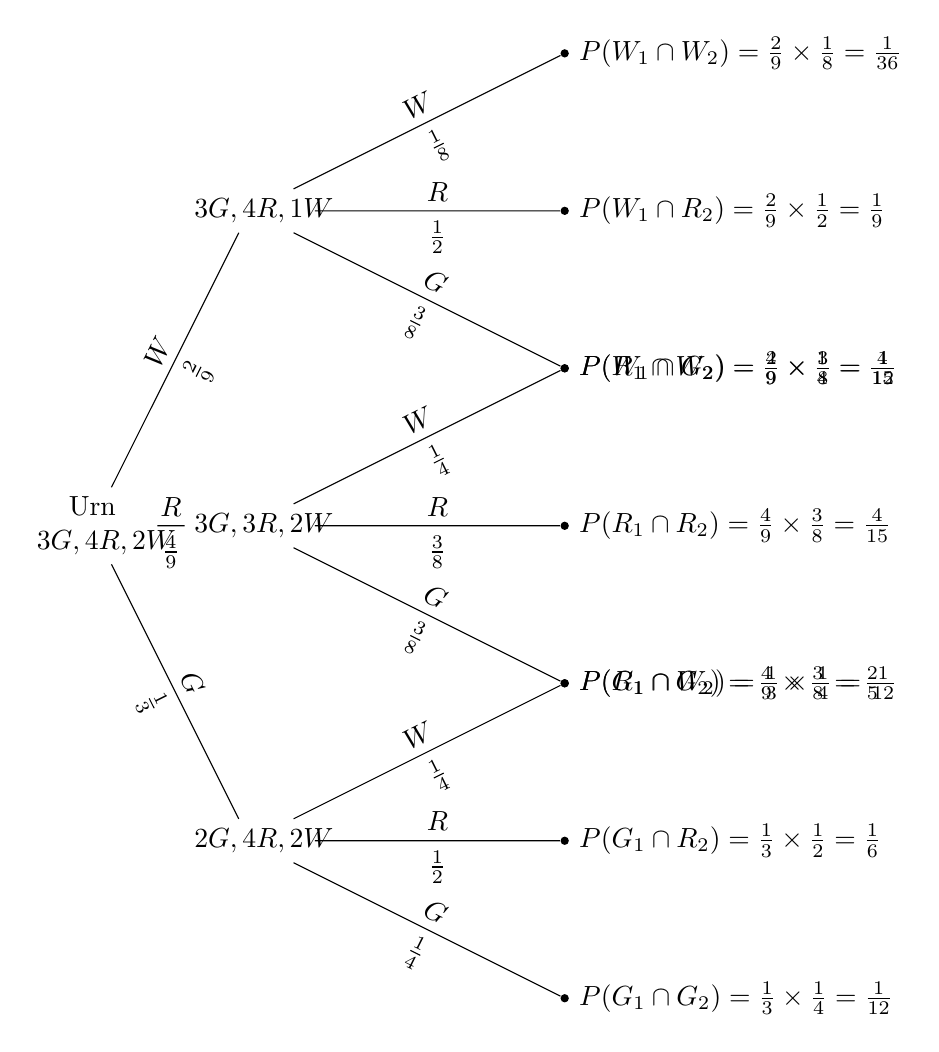
\begin{tikzpicture}[grow=right, sloped]
\node[bag] {Urn $3G, 4R, 2W$}
    child {
        node[bag] {$2G, 4R, 2W$}        
            child {
                node[end, label=right: {$P(G_1\cap G_2)=\frac{1}{3}\times\frac{1}{4}=\frac{1}{12}$}] {}
                edge from parent
                node[above] {$G$}
                node[below]  {$\frac{1}{4}$}
            }
            child {
                node[end, label=right: {$P(G_1\cap R_2)=\frac{1}{3}\times\frac{1}{2}=\frac{1}{6}$}] {}
                edge from parent
                node[above] {$R$}
                node[below]  {$\frac{1}{2}$}
            }
            child {
                node[end, label=right: {$P(G_1\cap W_2)=\frac{1}{3}\times\frac{1}{4}=\frac{1}{12}$}] {}
                edge from parent
                node[above] {$W$}
                node[below]  {$\frac{1}{4}$}
            }
            edge from parent 
            node[above] {$G$}
            node[below]  {$\frac{1}{3}$}
    }
    child {
        node[bag] {$3G, 3R, 2W$}   
            child {
                node[end, label=right: {$P(R_1\cap G_2)=\frac{4}{9}\times\frac{3}{8}=\frac{2}{5}$}] {}
                edge from parent
                node[above] {$G$}
                node[below]  {$\frac{3}{8}$}
            }
            child {
                node[end, label=right: {$P(R_1\cap R_2)=\frac{4}{9}\times\frac{3}{8}=\frac{4}{15}$}] {}
                edge from parent
                node[above] {$R$}
                node[below]  {$\frac{3}{8}$}
            }
            child {
                node[end, label=right: {$P(R_1\cap W_2)=\frac{4}{9}\times\frac{1}{4}=\frac{4}{15}$}] {}
                edge from parent
                node[above] {$W$}
                node[below]  {$\frac{1}{4}$}
            }
            edge from parent 
            node[above] {$R$}
            node[below]  {$\frac{4}{9}$}
    }
    child {
        node[bag] {$3G, 4R, 1W$}   
            child {
                node[end, label=right: {$P(W_1\cap G_2)=\frac{2}{9}\times\frac{3}{8}=\frac{1}{12}$}] {}
                edge from parent
                node[above] {$G$}
                node[below]  {$\frac{3}{8}$}
            }
            child {
                node[end, label=right: {$P(W_1\cap R_2)=\frac{2}{9}\times\frac{1}{2}=\frac{1}{9}$}] {}
                edge from parent
                node[above] {$R$}
                node[below]  {$\frac{1}{2}$}
            }
            child {
                node[end, label=right: {$P(W_1\cap W_2)=\frac{2}{9}\times\frac{1}{8}=\frac{1}{36}$}] {}
                edge from parent
                node[above] {$W$}
                node[below]  {$\frac{1}{8}$}
            }
            edge from parent         
            node[above] {$W$}
            node[below]  {$\frac{2}{9}$}
    };
\end{tikzpicture}


% Set the overall layout of the tree
\tikzstyle{level 1}=[level distance=1.5cm, sibling distance=2cm]
\tikzstyle{level 2}=[level distance=1.5cm, sibling distance=1cm]
\tikzstyle{level 3}=[level distance=4.5cm, sibling distance=.5cm]

% Define styles for bags and leafs
\tikzstyle{bag} = [text width=2em, text centered]
\tikzstyle{end} = [circle, minimum width=3pt,fill, inner sep=0pt]

\begin{tikzpicture}[grow=right, sloped]
\node {}
    child {
        node[bag] {$X$}  
            child {
                node {$X$}{}
            		child {
            		node {$X \qquad \textcolor{gris}{XXX} \quad 2\cdot 2 \cdot 2 = 8 \text{ posib.}$}
            		}
            		child {
            		node {$C  \qquad \textcolor{gris}{XXC} $}
            		}
            }
            child {
                node {$C$}{}
            		child {
            		node {$X  \qquad \textcolor{gris}{XCC} $}
            		}
            		child {
            		node {$C  \qquad \textcolor{gris}{XCX} $}
            		}
            }
    }
    child {
        node[bag] {$C$}   
            child {
                node {$X$} {}
                	child {
            		node {$X  \qquad \textcolor{gris}{CXX} $}
            		}
            		child {
            		node {$C  \qquad \textcolor{gris}{CXC} $ }
            		}
            }
            child {
                node {$C$} {}
               		child {
            		node {$X  \qquad \textcolor{gris}{CCX} $}
            		}
            		child {
            		node {$C  \qquad \textcolor{gris}{CCC} $}
            		}
            } 
    }
    ;
\end{tikzpicture}

\section{Líneas}
Linea gruesa degradada

	
\begin{tikzpicture}
	\fill [left color=black!30, right color=white] (0,0) rectangle (11.5,.1);
	\end{tikzpicture}
	
		
\begin{tikzpicture}
	\fill [left color=orange!30, right color=orange!5] (0,0) rectangle (11.5,.1);
	\end{tikzpicture}
	
	
Líneas sseparación


{\color{gris}\hrule}


\rule{50mm}{0.1mm}

\textcolor{gris}{\rule{50mm}{0.1mm}}

\begin{flushright}
\vspace{-10mm}\textcolor{gris}{\rule{100mm}{0.1mm}}	
\end{flushright}

\textcolor{red}{\rule{50mm}{0.1mm}}
	
\newpage
\section{Intento árbol esquema}





\begin{small}	

% Set the overall layout of the tree
\tikzstyle{level 1}=[level distance=2.5cm, sibling distance=4cm]
\tikzstyle{level 2}=[level distance=3cm, sibling distance=2cm]
\tikzstyle{level 3}=[level distance=3cm, sibling distance=1cm]


% Define styles for bags and leafs
\tikzstyle{bag} = [text width=4em, text centered]
\tikzstyle{end} = [circle, minimum width=3pt,fill, inner sep=0pt]

\begin{tikzpicture}[grow=right, sloped]

\node[bag] {?`Influye el orden?}
    child {
        node[bag] {?`Se pueden repetir?}        
            child {
                node[bag] {$CR_n^r=$\tiny{$\mqty(n+r-1\\r)$}}
                edge from parent
                node[above] {}
                node[below]  {NO}
            }
            child {
                node[bag] {$C_n^r=$\tiny{$\mqty(n\\r)$}}
                edge from parent
                node[above] {SÍ}
                node[below]  {}
            }
            edge from parent 
            node[above] {}
            node[below]  {NO}
    }
    % Primera rama
    child {
        node[bag] {?`Todos los elementos?}   
            child {
                node[bag] {?`Se pueden repetir?}
                		child {
            			node {$VR_n^r=n^r$}
            			}
            			child {
            			node {$V_n^r=\dfrac{n!}{(n-r)!}$}
            			}
                edge from parent
                node[above] {NO}
                node[below]  {}
            }
            child {
                node[bag] {?`Se pueden repetir?}
                		child {
            			node {$PR_n^{n_1,n_2,\cdots}=$\tiny{$\dfrac{n!}{n_1!\cdot n_2! \cdots}$}}
            			}
            			child {
            			node {$P_n=n!$}
            			}
                edge from parent
                node[above] {SÍ}
                node[below]  {}
            }
            edge from parent         
            node[above] {SÍ}
            node[below]  {}	
    };
\end{tikzpicture}

\end{small}

\vspace{2cm}

% Set the overall layout of the tree
\tikzstyle{level 1}=[level distance=2cm, sibling distance=4cm]
\tikzstyle{level 2}=[level distance=4cm, sibling distance=2cm]
\tikzstyle{level 3}=[level distance=5cm, sibling distance=1cm]


% Define styles for bags and leafs
\tikzstyle{bag} = [text width=4em, text centered]
\tikzstyle{end} = [circle, minimum width=3pt,fill, inner sep=0pt]

\begin{tikzpicture}[grow=right, sloped]

\node[bag] {?`Influye el orden?}
    child {
        node[bag] {?`Se pueden repetir?}        
            child {
                node[bag] {$CR_n^r=$\tiny{$\mqty(n+r-1\\r)$}}
                edge from parent
                node[above] {}
                node[below]  {NO}
            }
            child {
                node[bag] {$C_n^r=$\tiny{$\mqty(n\\r)$}}
                edge from parent
                node[above] {SÍ}
                node[below]  {}
            }
            edge from parent 
            node[above] {}
            node[below]  {NO}
    }
    % Primera rama
    child {
        node[bag] {?`Todos los elementos?}   
            child {
                node[bag] {?`Se pueden repetir?}
                		child {
            			node {$VR_n^r=n^r$}
            			edge from parent
                			node[above] {}
               				node[below] {SI}
            			}
            			child {
            			node {$V_n^r=\dfrac{n!}{(n-r)!}$}
            			edge from parent
                			node[above] {NO}
               				node[below] {}
            			}
                edge from parent
                node[above] {NO}
                node[below]  {}
            }
            child {
                node[bag] {?`Se pueden repetir?}
                		child {
            			node {$PR_n^{n_1,n_2,\cdots}=$\tiny{$\dfrac{n!}{n_1!\cdot n_2! \cdots}$}}
            				edge from parent
                			node[above] {}
               				node[below] {SI}
            			}
            			child {
            			node {$P_n=n!$}
            				edge from parent
                			node[above] {NO}
               				node[below] {}
            			}
                edge from parent
                node[above] {SÍ}
                node[below]  {}
            }
            edge from parent         
            node[above] {SÍ}
            node[below]  {}	
    };
\end{tikzpicture}

\newpage

\section{histogramas tikz}


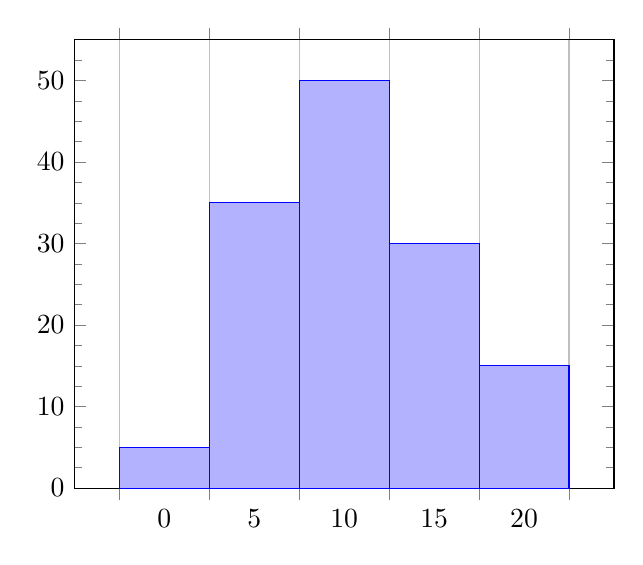
\begin{tikzpicture}
\begin{axis}[ybar interval, ymax=55,ymin=0, minor y tick num = 3]
\addplot coordinates { (0, 5) (5, 35) (10, 50) (15, 30) (20, 15) (25, 0) };
\end{axis}
\end{tikzpicture}

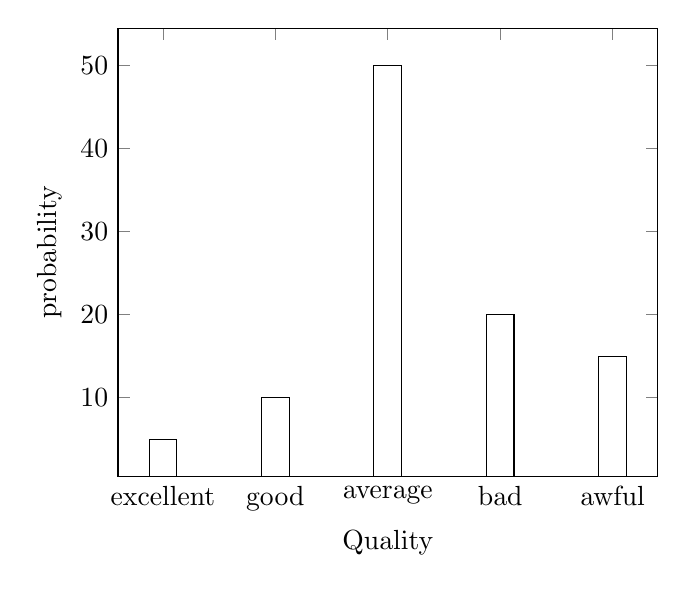
\begin{tikzpicture}
\begin{axis}[
    symbolic x coords={excellent, good, average, bad, awful},
        ylabel = {probability},
        xlabel = {Quality},
    xtick=data]
    \addplot[ybar,fill=white] coordinates {
        (excellent,5)
        (good,10)
        (average,50)
    (bad, 20)
    (awful,15)
    };
\end{axis}
\end{tikzpicture}	


\section{lineas horzontales}




